\section{Databricks Light vs. EMR Presto}\label{databricksLight}

In this section, we compare EMR Presto with Databricks Light. Based on the open source Apache Spark framework, Databricks Light offers an alternative to the Databricks Data Engineering runtime; hence, it is also referred to as Data Engineering Light. The price per hour for operating Databricks Light clusters is about half that of Databricks Data Engineering, but it lacks the advanced performance and reliability features of the latter. An additional restriction is that Databricks Light can only be used for job clusters and not for interactive clusters.

Concretely, the experiments in this section use the Light 2.4 runtime instead of the 5.3 runtime of our reference results, both of which employ Spark 2.4 and Scala 2.11.

\subsection{Data loading}

The results of the Data Loading Test appear in Figure \ref{fig:prestoVsDatabricksLightDataLoadingTotalTime}. Databricks Light is about 50\% slower than EMR Presto using the ORC format, and about twice as slow as Databricks Data Engineering. Clearly, data loading is far from being a straightforward task, and an optimized implementation can yield major performance improvements. In terms of monetary costs (summarized in Section \ref{resultsSummaryTotalCost}), EMR Presto and Databricks Data Engineering are close to balancing each other, while Databricks Light is more than 30\% more expensive.

\begin{figure}
   \begin{center}
   \scalebox{0.65}{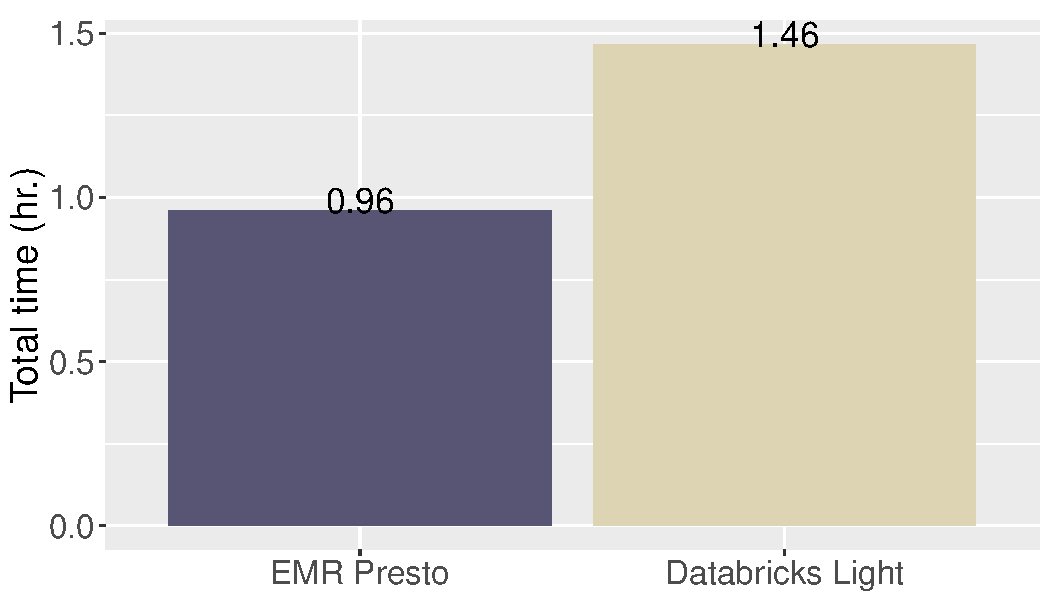
\includegraphics[width=7.0in]{imgs/databricksLight/load_totalHrTimeBarChart.pdf}}
   \end{center}
   \caption{EMR Presto vs. Databricks Light Data Loading Test total time.}
   \label{fig:prestoVsDatabricksLightDataLoadingTotalTime}
\end{figure}

\subsection{Individual query execution (Power Test)}

We present the metrics associated with the Power Test in Figure \ref{fig:prestoVsDatabricksLightPowerTestTotalTime} to Figure \ref{fig:prestoVsDatabricksLightPowerTestArithmeticMean}. Overall, EMR Presto and Databricks Light show a very similar performance.

\begin{figure}
   \begin{center}
   \scalebox{0.65}{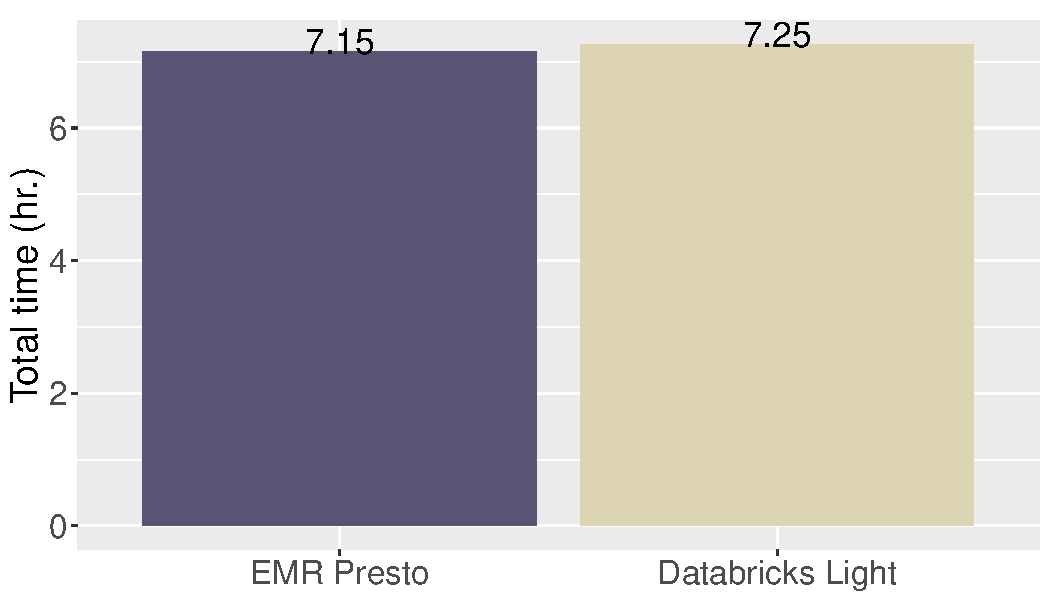
\includegraphics[width=7.0in]{imgs/databricksLight/power_totalHrTimeBarChart.pdf}}
   \end{center}
   \caption{EMR Presto vs. Databricks Light Power Test total time.}
   \label{fig:prestoVsDatabricksLightPowerTestTotalTime}
\end{figure}

\begin{figure}
   \begin{center}
   \scalebox{0.65}{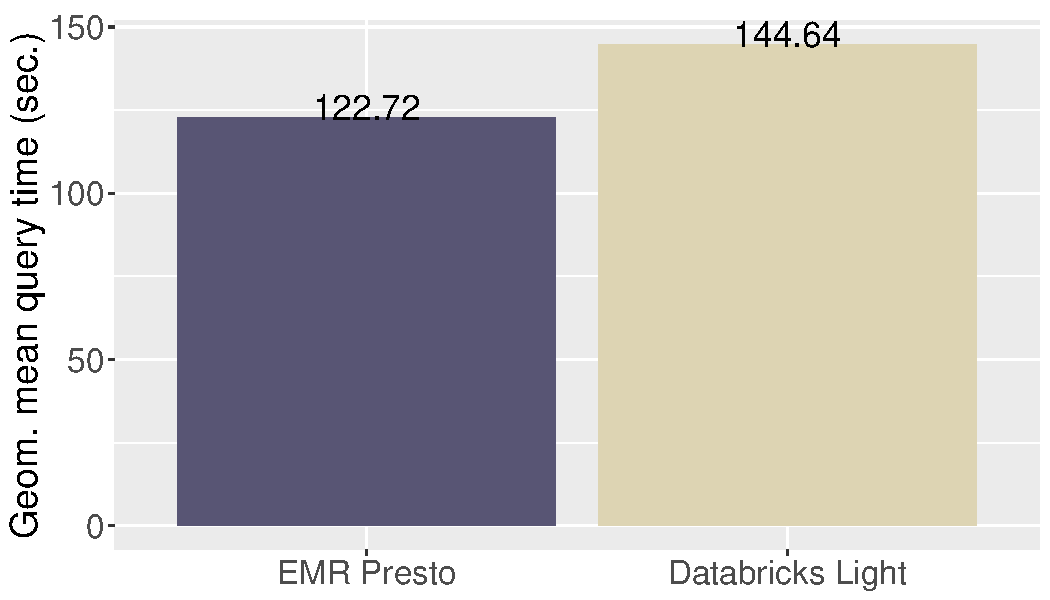
\includegraphics[width=7.0in]{imgs/databricksLight/power_geomeanTimeBarChart.pdf}}
   \end{center}
   \caption{EMR Presto vs. Databricks Light Power Test query execution time geometric mean.}
   \label{fig:prestoVsDatabricksLightPowerTestGeomean}
\end{figure}

\begin{figure}
   \begin{center}
   \scalebox{0.65}{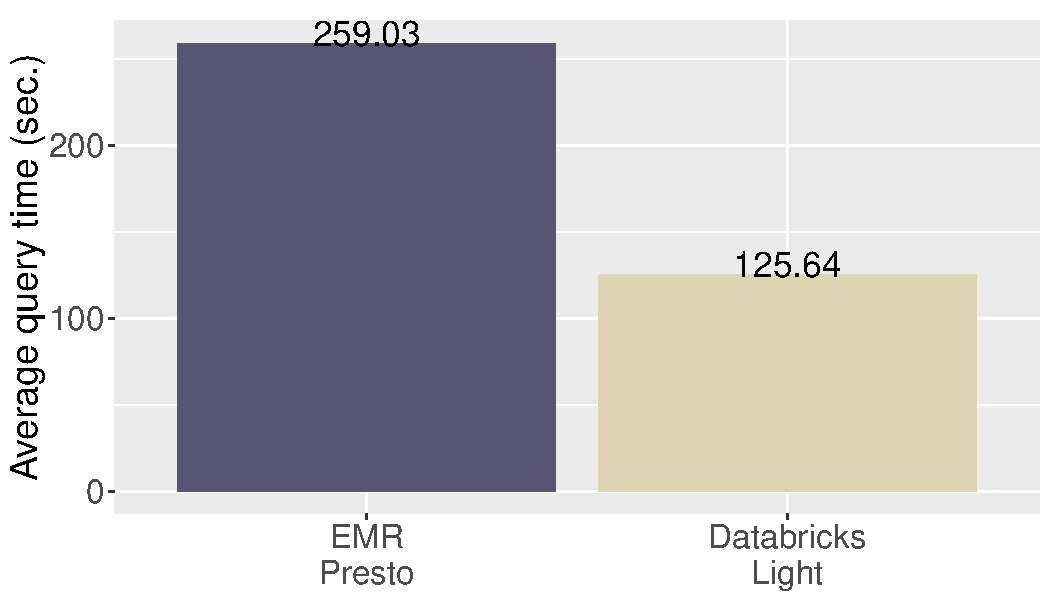
\includegraphics[width=7.0in]{imgs/databricksLight/power_avgTimeBarChart.pdf}}
   \end{center}
   \caption{EMR Presto vs. Databricks Light Power Test query execution time arithmetic mean.}
   \label{fig:prestoVsDatabricksLightPowerTestArithmeticMean}
\end{figure}

The comparison of individual queries that we show in Figure \ref{fig:prestoVsDatabricksLightPowerTestIndividualQueries1} to Figure \ref{fig:prestoVsDatabricksLightPowerTestIndividualQueries5} enables to make a more in depth analysis. Databricks Light gives a better performance in 36 queries, while the remaining 63 favor EMR Presto. Among the queries that complete faster in Databricks Light, 23 of them do so by a margin of 25\% or more. In the case of the queries that are faster in EMR Presto, 51 of them are at least 25\% faster. In general, Databricks Light is significantly faster for a subset of the queries in the benchmark, while EMR Presto is significantly faster for the larger complementary subset.

\begin{figure}
   \begin{center}
   \scalebox{0.65}{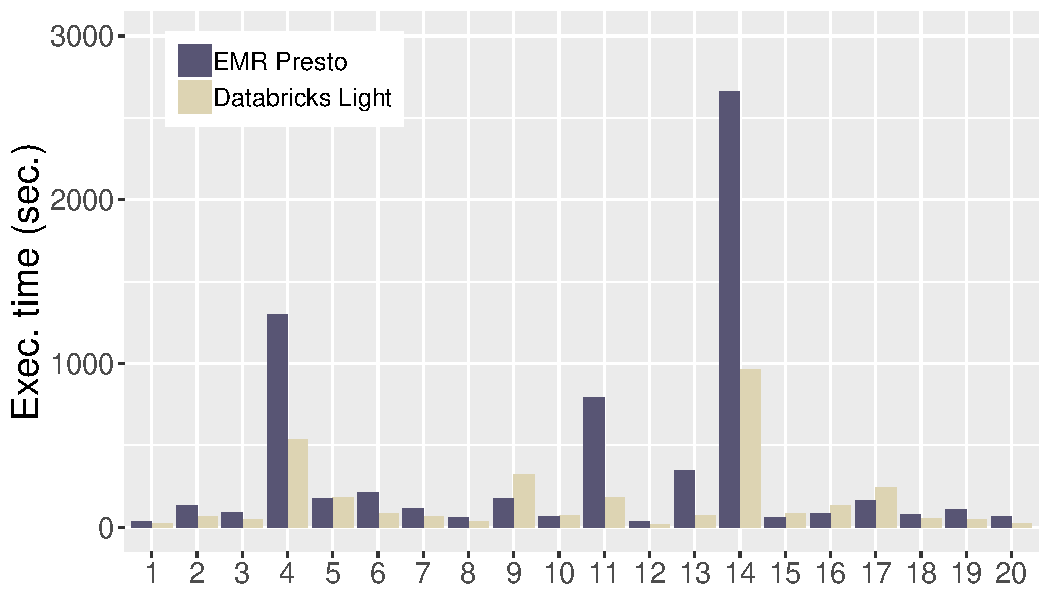
\includegraphics[width=7.0in]{imgs/databricksLight/1_PDFsam_PowerTestCompAll.pdf}}
   \end{center}
   \caption{EMR Presto vs. Databricks Light Power Test individual query times (1).}
   \label{fig:prestoVsDatabricksLightPowerTestIndividualQueries1}
\end{figure}

\begin{figure}
   \begin{center}
   \scalebox{0.65}{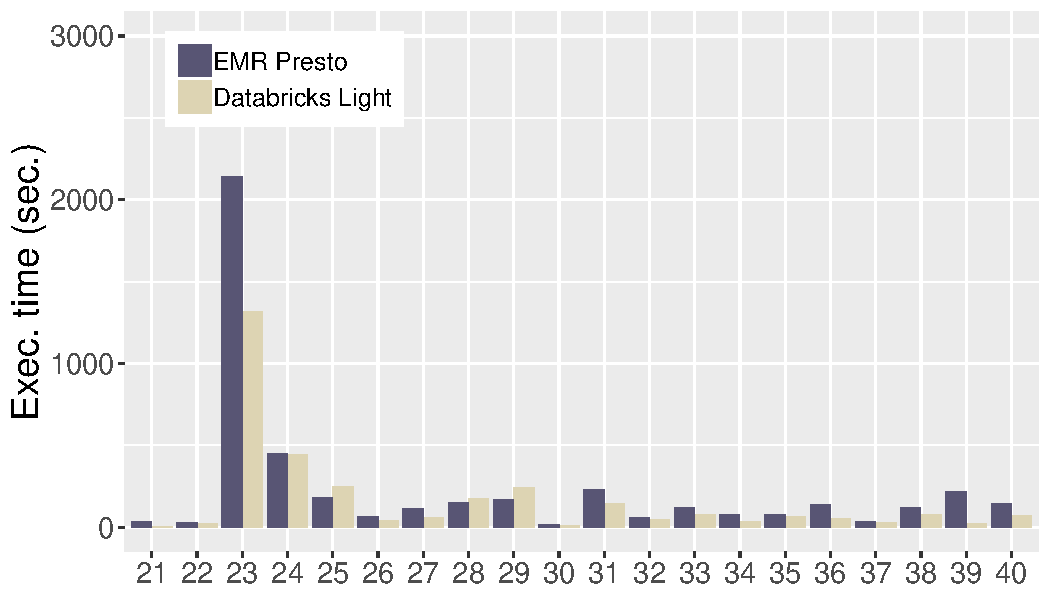
\includegraphics[width=7.0in]{imgs/databricksLight/2_PDFsam_PowerTestCompAll.pdf}}
   \end{center}
   \caption{EMR Presto vs. Databricks Light Power Test individual query times (2).}
   \label{fig:prestoVsDatabricksLightPowerTestIndividualQueries2}
\end{figure}

\begin{figure}
   \begin{center}
   \scalebox{0.65}{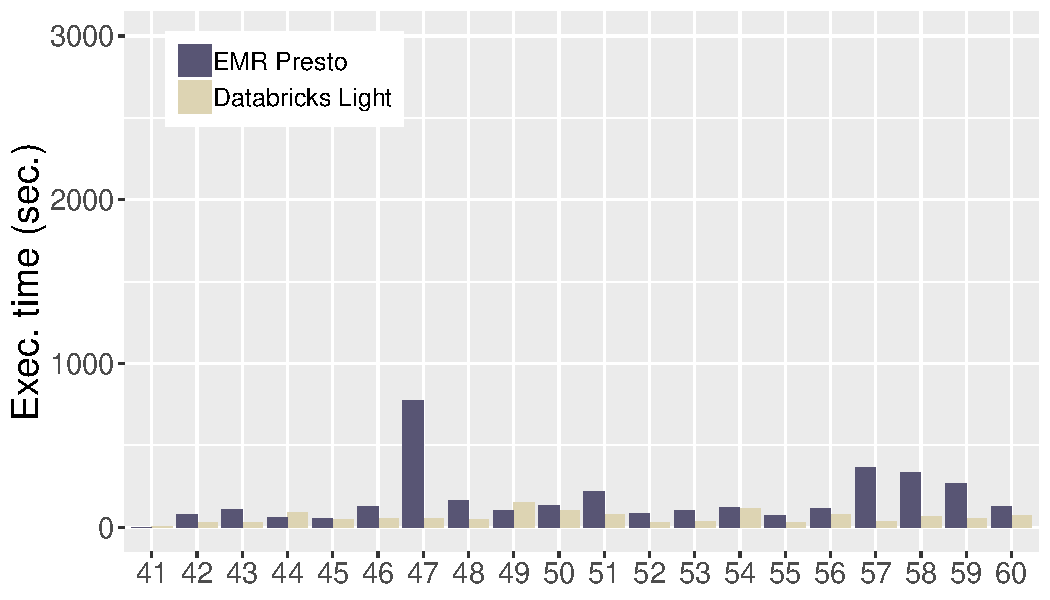
\includegraphics[width=7.0in]{imgs/databricksLight/3_PDFsam_PowerTestCompAll.pdf}}
   \end{center}
   \caption{EMR Presto vs. Databricks Light Power Test individual query times (3).}
   \label{fig:prestoVsDatabricksLightPowerTestIndividualQueries3}
\end{figure}

\begin{figure}
   \begin{center}
   \scalebox{0.65}{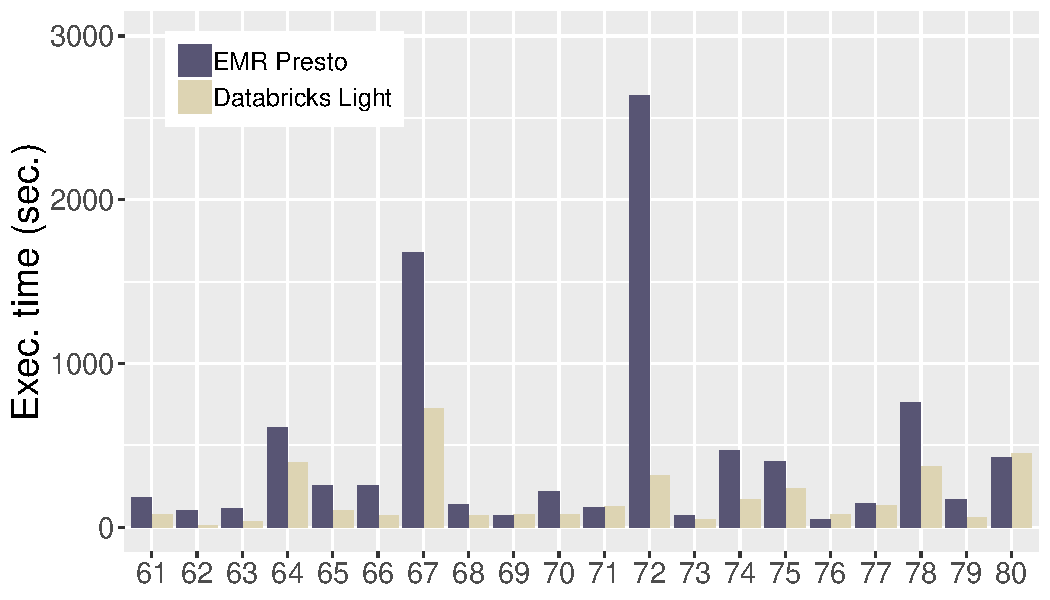
\includegraphics[width=7.0in]{imgs/databricksLight/4_PDFsam_PowerTestCompAll.pdf}}
   \end{center}
   \caption{EMR Presto vs. Databricks Light Power Test individual query times (4).}
   \label{fig:prestoVsDatabricksLightPowerTestIndividualQueries4}
\end{figure}

\begin{figure}
   \begin{center}
   \scalebox{0.65}{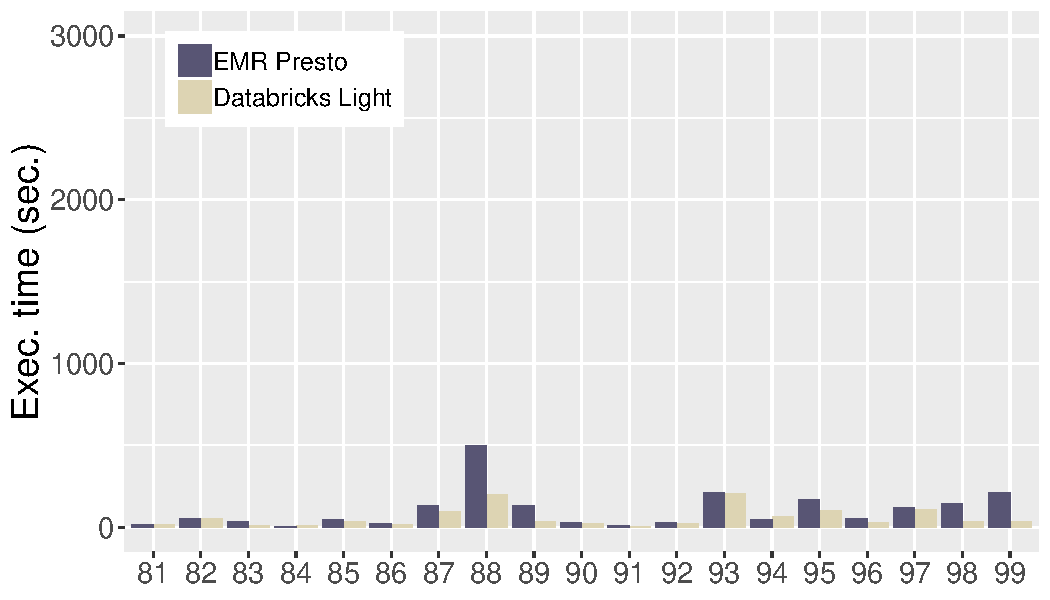
\includegraphics[width=7.0in]{imgs/databricksLight/5_PDFsam_PowerTestCompAll.pdf}}
   \end{center}
   \caption{EMR Presto vs. Databricks Light Power Test individual query times (5).}
   \label{fig:prestoVsDatabricksLightPowerTestIndividualQueries5}
\end{figure}

If we were to exclude query 72, which is much slower in EMR Presto, the performance of Databricks Light in relation to the total time required for the Power Test would be about 10\% worse than EMR Presto. This is partially reflected in the geometric mean in contrast to the arithmetic mean, shown in Figure \ref{fig:prestoVsDatabricksLightPowerTestGeomean} and Figure \ref{fig:prestoVsDatabricksLightPowerTestArithmeticMean}, respectively.

\subsection{Concurrent query execution (Throughput Test)}

We provide the results for the Throughput Test in Figure \ref{fig:prestoVsDatabricksLightTputTest}. Databricks Light outperforms EMR Presto by a small margin of about 8\%.

\begin{figure}
   \begin{center}
   \scalebox{0.65}{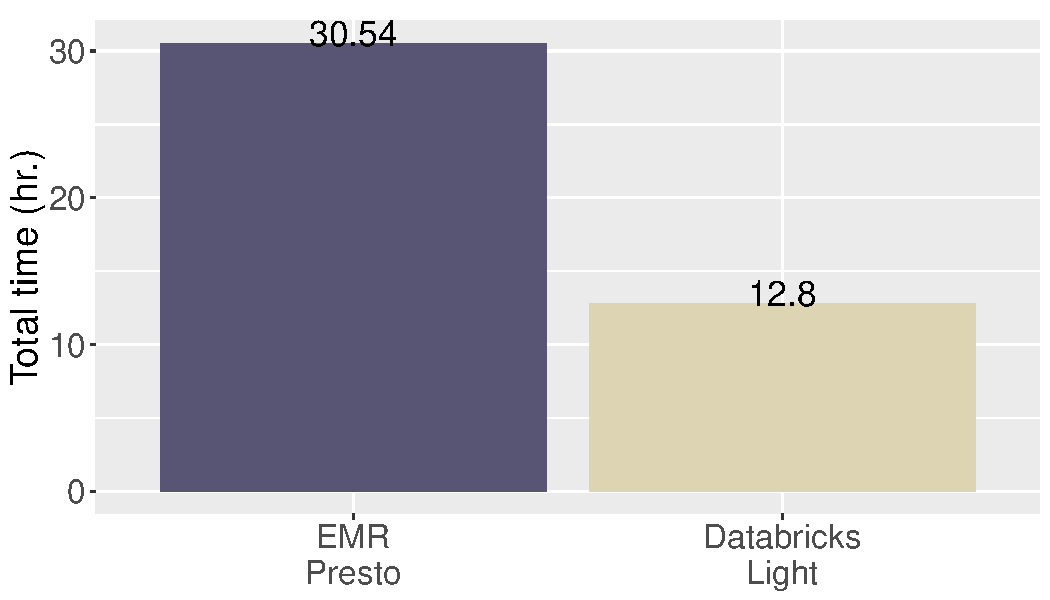
\includegraphics[width=7.0in]{imgs/databricksLight/tput_totalHrTimeBarChart.pdf}}
   \end{center}
   \caption{EMR Presto vs. Databricks Light Throughput Test total time.}
   \label{fig:prestoVsDatabricksLightTputTest}
\end{figure}

Again, the performance of Databricks Light and EMR Presto is very similar. Even in total costs, as we show in Section \ref{resultsSummaryTotalCost}, the benchmark results are close. Given that running a job either on Databricks Light or in Databricks Data Engineering requires minimal configuration changes, it is definitely an advantage to have two alternatives with distinct price-performance profiles; we provide the concrete metrics in Section \ref{resultsSummaryPerformanceMetric}.



